\chapter{Marco te\'orico}\label{capit:cap2}
\vspace{-2.0325ex}%
\noindent
\rule{\textwidth}{0.5pt}
\vspace{-5.5ex}% 
\newcommand{\pushline}{\Indp}% Indent puede ir o no :p

\section{Gestos}\label{sec:2Gestos}
Los gestos \citep{Mitra2007} son movimientos del cuerpo expresivos y significativos que involucran dedos, manos, brazos, cabeza, cara o cuerpo con la intención de transmitir información relevante o interactuar con el ambiente. De acuerdo con la literatura \citep{Mitra2007} los gestos con las manos se clasifican en estáticos y dinámicos, los primeros están definidos como la posición y orientación de la mano en el espacio manteniendo esta pose durante cierto tiempo, por ejemplo para hacer una se\~nal de aventón, a diferencia de los gestos dinámicos donde hay movimiento de la pose, un ejemplo  es cuando mueves la mano en se\~nal de adiós. De aquí en adelante entiéndase el término gestos con las manos, como gestos.  

\section{Reconocimiento de gestos con la manos}\label{sec:2ReconocimientoGestos}  

El reconocimiento de gestos es 

El reconocimiento de gestos se divide en tres fases \citep{Rautaray2012}, detección o segmentación; extracci\'on de caracter\'isticas seguimiento; dependiendo si los gestos son dinámicos, por último la etapa final el reconocimiento del gesto.  
Este se clasifican en dos modelos, basados en la visi\'on y en contacto, esta clasificaci\'on depende de la manera en que son capturados los datos, es decir la forma en que se obtiene el gesto, para posteriormente poderlo reconocer. 

Los primeros acercamientos para llevar acabo el reconocimiento de gestos fue usando modelos de contacto \citep{Rautaray2012} y \citep{Nayakwadi2014}, como su nombre lo dice utilizan dispositivos que est\'an en contacto f\'isico con la mano del usuario, esto para capturar el gesto a reconocer, por ejemplo existen guantes de datos, marcadores de colores, acelerómetros y pantallas multi-touch, aunque estos no son tan aceptados pues entorpecen la naturalidad entre la interacción del humano y la computadora. Los modelos basados en la visi\'on surgieron como respuesta a esta desventaja, estos utilizan cámaras para extraer la información necesaria para realizar el reconocimiento, los dispositivos van desde c\'amaras web hasta algunas más sofisticadas por ejemplo c\'amaras de profundida.  

En este trabajo, se toma el enfoque basado en la visi\'on ya que se quiere obtener un sistema que para el usuario sea fácil de interactuar, y esta interacci\'on sea natural y una manera de lograr esto es tomando este enfoque.  estos tienen mayor complejidad (acomodar este parrafo :P)


Los métodos basados en la visión se pueden representar por dos modelos \citep{Rautaray2012}, los basados en 3D, da una descripción espacial en 3D de la mano, y los basados en apariencia, como su nombre lo dice se basan en la apariencia de la mano. Los modelos basados en apariencia se dividen en dos categorías, los estáticos (modelo de silueta, de contorno deformables) y de movimiento (de color y movimiento).

\subsection{Etapas del reconocimiento de gestos}\label{subsec:EtapasReconocimiento} 
Enseguida se describen las etapas del reconocimiento de gestos (detección, seguimiento y reconocimiento), con los métodos para llevar cada una de estas.  



\subsubsection{Detección}\label{sssec:EtapaDeteccion}

En esta etapa se detecta y segmenta la información relevante de la imagen (la mano), con la del fondo, existen distintos métodos para obtener dichas características como la de color de la piel, forma, movimiento, entre otras que generalmente son combinaciones de alguna de estas, para obtener un mejor resultado. Enseguida se describe brevemente cada una de estas.  
\begin{itemize}
\item Color de la piel: Se basa principalmente en escoger un espacio del color, es una organización de colores especifica; como; RGB (rojo, verde, azul), RG (rojo, green), YCrCb (brillo, la diferencia entre el brillo y el rojo, la diferencia entre el brillo y el azul), etc. La desventaja es que si es color de la piel es similar al fondo, la segmentación no es buena, la forma de corregir esta segmentación es suponiendo que el fondo no se mueve con respecto a la cámara.
\item Forma: Extrae el contorno de las imágenes, si se realiza correctamente se obtiene el contorno de la mano. Aunque si se toman las yemas de los dedos como características, estas pueden ser ocluidas por el resto de la mano, una posible solución es usar más de una cámara.  
\item Valor de p\'ixeles: Usar imágenes en tonos de gris para detectar la mano en base a la apariencia y textura, esto se logra entrenando un clasificador con un conjunto de imágenes.
	\item Modelo 3D: Depende de cual modelo se utilice, son las características de la mano requeridas. 
	\item Movimiento: Generalmente esta se usa con otras formas de detección ya que para utilizarse por sí sola hay que asumir que el único objeto con movimiento es la mano.
\end{itemize}

\subsubsection{Seguimiento}\label{sssec:EtapaSeguimiento}

Consiste en localizar la mano en cada cuadro (imagen). Se lleva acabo usando los métodos de detección si estos son lo suficientemente rápidos para detectar la mano cuadro por cuadro. Se explica brevemente los métodos para llevar a cabo el seguimiento. 
\begin{itemize}
	\item Basado en plantillas: Este se divide en dos categorías (Características basadas en su correlación y basadas en contorno), que son similares a los métodos de detección, aunque supone que las imágenes son adquiridas con la frecuencia suficiente para llevar acabo el seguimiento. Características basadas en su correlación, sigue las características a través de cada cuadro, se asume que las características aparecen en mismo vecindario. Basadas en contorno, se basa en contornos deformables, consiste en colocar el contorno cerca de la región de interés e ir deformando este hasta encontrar la mano. 
	\item Estimación óptima: Consiste en usar filtros Kalman, un conjunto de ecuaciones matemáticas que proporciona una forma  computacionalmente eficiente y recursiva de estimar el estado de un proceso, de una manera que minimiza la media de un error cuadrático, el filtro soporta estimaciones del pasado, presente y futuros estados, y puede hacerlo incluso cuando la naturaleza precisa del modelo del sistema es desconocida;  para hacer la detección de características en la trayectoria. 
	\item Filtrado de partículas: Un método de estimación del estado de un sistema que cambia a lo largo del tiempo, este se compone de un conjunto de partículas (muestras) con pesos asignados, las partículas son estados posibles del proceso. Es utilizado cuando no se distingue bien la mano en la imagen. Por medio de partículas localiza la mano la desventaja es que se requieren demasiadas partículas, y el seguimiento se vuelve imposible. 
	\item Camshift: Busca el objetivo, en este caso la mano, encuentra el patrón de distribución mas similar en una secuencia de imágenes, la distribución puede basada en el color. 
\end{itemize}

\subsubsection{Reconocimiento}\label{sssec:EtapaReconocimiento}

Es la clasificación del gesto, la etapa final del reconocimiento, la clasificación se puede hacer dependiendo del gesto. Para gestos estáticos basta con usar algún clasificador o empatar el gesto con una plantilla. En los dinámicos se requiere otro tipo de algoritmos de aprendizaje de máquina. A continuación se encuentran los principales métodos para llevar acabo el reconocimiento del gestos. 
\begin{itemize}
	\item K-medias: Consiste en determinar los $k$ puntos llamados centros para minimizar el error de agrupamiento, que es la suma de las distancias de todo los puntos al centro de cada grupo. El algoritmo empieza localizando aleatoriamente $k$ grupos en el espacio espectral. Cada p\'ixel en la imagen de entrada es entonces asignadas al centro del grupo mas cercano  
	\item {K-vecinos cercanos} (KNN, por sus siglas en ingl\'es): 
	Este es un método para clasificar objetos basado en las muestras de entrenamiento en el espacio de características. 
	\item Desplazamiento de medias: Es un método iterativo que encuentra el máximo en una función de densidad dada una muestra estadística de los datos.
	\item Máquinas de soporte vectorial (SVM, por sus siglas en ingl\'es). Consiste en un mapeo no lineal de los datos de entrada a un espacio de dimensi\'on m\'as grande, donde los datos pueden ser separados de forma lineal.  
	\item Modelo oculto de Markov (HMM, por sus siglas en ingl\'es) es definido como un conjunto de estados donde un estado es el estado inicial, un conjunto de símbolos de salida y un conjunto de estados de transición. En el reconocimiento de gestos se puede caracterizar a    los estados como un conjunto de las posiciones de la mano; las  transiciones de los estados como la probabilidad de transición de cierta posición de la mano a otra; el símbolo de salida como una postura especifica y la secuencia de los símbolos de salida como  el gesto de la mano.   
	\item Redes neuronales con retraso: Son una clase de redes neuronales artificiales que se enfocan en datos continuos, haciendo que el sistema sea adaptable para redes en linea y les da ventajas sobre aplicaciones en tiempo real. 
\end{itemize}  


\section{Imagen}\label{ImagenDef} 

Una imagen se puede definir como una función bidimensional, $S(x,y)$ donde $x$, $y$ representan las coordenadas en el plano y el valor de la función es la intensidad o nivel de gris en el punto $(x,y)$. 
Si el valor de la función y los puntos de la imagen son finitos, esta es una imagen digital, la cual se puede representar en una matriz donde cada valor o pixel es el nivel de gris de la imagen, y los indices de esta indican la posición, \citep{Gonzalez2002}.


\section{Sensor Kinect}\label{KinectSensor} 

En noviembre del 2010 la compa\'nia Microsoft lanz\'o el sensor Kinect para consolas de vídeo juego Xbox 360 y en febrero del 2011 lanz\'o la versi\'on para Windows, que se muestra en la figura \ref{fig:KinectPic}.  

El dispositivo Kinect esta equipado con una serie de sensores que permiten obtener imágenes a color y de profundidad (imágenes que indican a la distancia que esta un objeto del sensor), los cuales permiten hacer detección y seguimiento de personas. Detecta $6$ personas y hace el seguimiento de $2$ personas \footnote{https://msdn.microsoft.com/en-us/library/hh973074.aspx}.    
  
\begin{figure}[h!]
\begin{center}
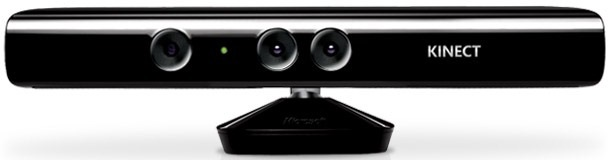
\includegraphics[scale=.6]{./Figures/Kinect.jpg}
\end{center}
\caption{Sensor Kinect para Windows}
\label{fig:KinectPic}
\end{figure} 

El sensor esta equipado con los siguientes componentes: un cámara de color o sensor de color, un emisor infrarrojo, un sensor infrarrojo de profundidad, un motor que controla la inclinación, un arreglo de cuatro micrófonos y un LED \ref{fig:KinectComponentes}. 

\begin{figure}[!h]
\begin{center}
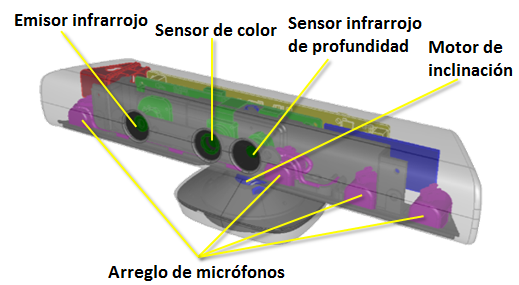
\includegraphics[scale=.6]{./Figures/sensor.png}
\end{center}
\caption{Componentes del sensor Kinect}
\label{fig:KinectComponentes}
\end{figure} 

Enseguida se describen brevemente cada uno de los componentes del sensor Kinect. 
\begin{itemize}
\item La cámara de color captura y transmite datos de vídeo a color, detectando los colores rojo, verde y azul (RGB, por sus siglas en ingl\'es, red, green and blue). La transmisión de datos que brinda la cámara es una secuencia de imágenes (cuadros), a una velocidad de hasta $30$ cuadros por segundo con una resolución de hasta $1280\, x \, 960$ p\'ixeles. La velocidad de los cuadros por segundo varia según la resolución de la imagen.  

\item El emisor infrarrojo proyecta puntos de luz infrarroja frente al sensor, con estos puntos y el sensor de profundidad se puede medir la profundidad que existe del sensor.

\item El sensor infrarrojo lee los puntos infrarrojos proyectados y calcula la distancia que existe entre el objeto y el sensor. El sensor transmite los datos de profundidad con una velocidad de $30$ cuadros por segundo con una resolución de hasta $640 \, x \, 480$ pixeles.   

\item El motor de inclinación controla el \'angulo de la posición vertical de los sensores del dispositivo. El motor puede moverse desde el \'angulo de $-27^ \circ$ a $+27^\circ$. 

\item Arreglo de micrófonos, consta de $4$ micrófonos, captura el sonido y localiza la dirección en la que proviene. 

\item LED indica el estado del sensor.
 
\end{itemize}


 
\section{Detección rápida de objetos usando características simples utilizando el clasificador de cascada impulsada}\label{sec:ViolaJones}

El m\'etodo  desarrollado por \citep{Viola2001} fue creado originalmente para atacar el problema de detección de rostros, este puede ser usando para detectar cualquier objeto, debido a la forma en que este fue creado, pues detecta un objeto clasificando imágenes basándose en el valor de características simples.

La técnica clasifica si el objeto se encuentra en la escena, usando AdaBoost en forma de cascada, y discrimina el objeto tomando en cuenta el valor de las características, se usan las características Haar, el valor de estas es calculado mediante una imagen integral.

(Parece que falta explicar mas el algoritmo de cascada) 

En seguida se explica a detalle cada etapa del método. 

\subsection{Características Haar}\label{subsec:CaracteristicasHaar}  

Las características Haar son operadores rectangulares como los de la figura \ref{fig:haarFeatures}.\\ 
Las características con dos rectángulos \ref{fig:haarFeatures:1}, \ref{fig:haarFeatures:2} , contienen dos regiones rectangulares adyacentes, y el valor de la característica se calcula tomando la diferencia de la suma de ambas regiones.\\ 
Las características con tres rectángulos \ref{fig:haarFeatures:3}, contienen tres regiones rectangulares adyacentes, y el valor de la característica se calcula la suma de las regiones exteriores y se resta la suma de la región interior.\\ 
Las características con cuatro rectángulos \ref{fig:haarFeatures:4}, contienen cuatro regiones rectangulares adyacentes, y el valor de la característica se obtiene con la diferencia entre las regiones pares diagonales.

\begin{figure}%[htbp]
\centering
\subfigure[]{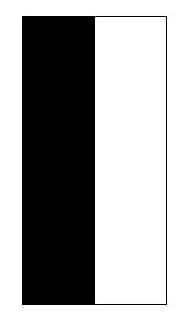
\includegraphics[scale=.4]{./Figures/haarFeatures1}\label{fig:haarFeatures:1}}
\subfigure[]{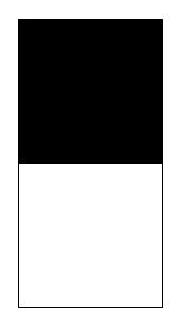
\includegraphics[scale=.4]{./Figures/haarFeatures2}\label{fig:haarFeatures:2}}
\subfigure[]{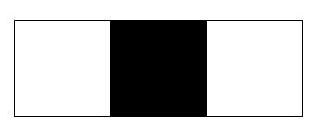
\includegraphics[scale=.4]{./Figures/haarFeatures3}\label{fig:haarFeatures:3}}
\subfigure[]{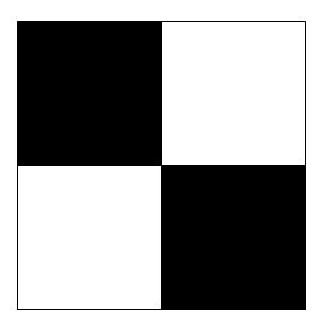
\includegraphics[scale=.4]{./Figures/haarFeatures4}\label{fig:haarFeatures:4}}
\caption{Ejemplo de operadores Haar} \label{fig:haarFeatures}
\end{figure}

\subsection{Imagen integral}\label{subsec:IntegralImage} 

Uno de los aportes de este método es el concepto de imagen integral con la cual se calcula el valor de las características. La imagen integral, $SI$, se calculada como la suma del valor de los pixeles que se encuentran arriba y a la izquierda de cierta posición.    

$$SI(x,y)=S(x,y) + S(x-1,y) + SI(x,y-1)-SI(x-1,y-1)$$ 

La imagen integral permite calcular la suma de los pixeles de cierta región usando solo los valores de las esquinas de dicha región, la cual se obtiene como:   

$$REG(\alpha)=SI(A)+SI(D)-SI(B)-SI(C)$$

donde $REG(\alpha)$ es la región a la cual se le quiere calcular el valor de la suma de sus pixeles; $A,B,C,D$ son las esquinas de dicha región, como se muestra en la figura \ref{fig:figImageIntegral}

\begin{figure}[!h]
\begin{center}
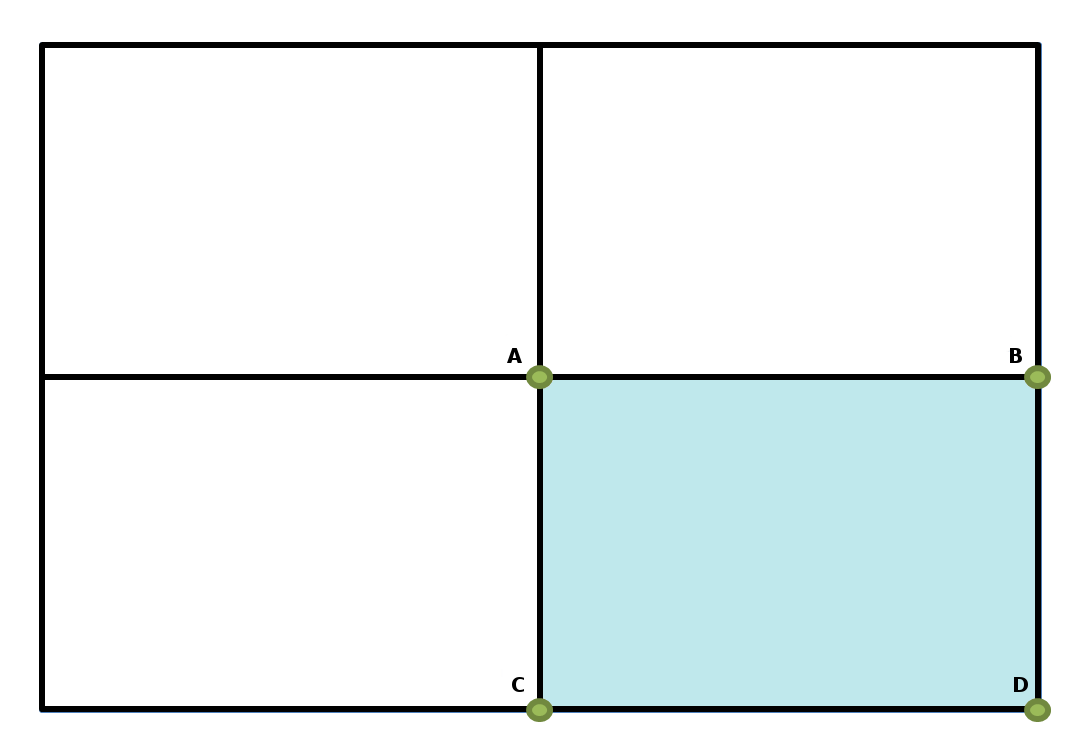
\includegraphics[scale=.3]{./Figures/IntegralImage.png}
\end{center}
\caption{Regiones de imagen integral}
\label{fig:figImageIntegral}
\end{figure} 

\subsection{Clasificador AdaBoost}\label{subsec:AdaboostClasifier}  

El algoritmo AdaBoost realiza su clasificación construyendo un clasificador fuerte $h(x)$ de clasificadores débiles $h_i(x)$. Los clasificares débiles son calculados de la siguiente manera: 

$$h_i(x)=
\begin{cases}   
1, \quad Si \quad  p_if_i<p_i \theta_i \\
0, \quad de \quad otra \quad forma.\\
\end{cases}$$

donde $f_i(x)$ es una característica, $\theta$ es un umbral, y $p_i(x)$ representa el signo de la desigualdad.   

El clasificador fuerte es una combinación lineal de los clasificadores débiles, y se define de la siguiente forma: 

$$h(x)= \alpha_1h_1(x)+\alpha_2h_2(x)+ \cdots +\alpha_nh_n(x)$$ 

donde $n$ es el n\'umero de características, $\alpha_i$ es el valor asociado a cada característica, el cual va entre $0$ y $1$.


\subsection{Clasificador AdaBoost en Cascada}\label{subsec:AdaboostCascade}   


\section{Binarización}\label{Binarization} 

La binarización es una técnica de procesamiento de imágenes, la cual se encarga de transformar una imagen en escala de grises $S(x,y)$ en una imagen binaria $B(x,y)$ es decir, los pixeles de la imagen toman un valor de $0$ ó $1$.   
Para formar la imagen binaria un valor, umbral, de la imagen en escala de grises es seleccionado. Ya que se tiene el umbral, $T$,     
los pixeles de la imagen son discriminados dependiendo si su valor es mayor o igual al umbral entonces el valor de los pixeles en la imagen binaria es $1$ el resto toma valor de $0$. Es decir: 

$$B(x,y)=
\begin{cases}   
1, \quad Si \quad  S(x,y)\geq T \\
0, \quad de \quad otra \quad forma.\\
\end{cases}$$

Existen diversas técnicas para binarizar una imagen, estas se pueden clasificar en dos grupos dependiendo de la manera es que es calcula el umbral, global o local. Los métodos globales calculan un umbral que es usado en toda la imagen y los métodos locales calculan varios umbrales para ciertas regiones de la imagen.  

Un método de binarización muy utilizado es el de NiBlack, \citep{Chaki2014} es un método local y adaptativo ya que adapta el umbral basándose en la media $m(i,j)=$ y la desviación estándar $\sigma(i,j)$ de una ventana deslizante de tamaño $bxb$. El umbral $T$  se calcula como: 

$$T(i,j)=m(i,j)+k \cdot \sigma(i,j)$$ 

donde $k \in [0,1]$ el valor de la constante determina que tanta parte del contorno es preservado.


  
\section{Operaciones Morfológicas}\label{OperacionesMorfologicas} 

Otra técnica muy utilizada en procesamiento de imágenes son las operaciones morfológicas que son un conjunto de operaciones no lineales, la idea es que al aplicar alguna de estas operaciones el ruido se removido tomando en cuanta la forma y estructura de la imagen. 
La operaciones morfológicas utilizan un elemento estructural el cual se aplica por toda la imagen, los elementos estructurales pueden ser de distintas formas como \ref{fig:EX}

\begin{figure}
\centering
\subfigure[Rectángulo de $3x3$.]{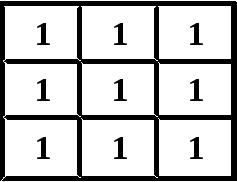
\includegraphics[scale=.7]{./Figures/EX1}\label{fig:EX:1}} %\hspace{20mm}
\qquad
\subfigure[Figura de $3x2$.]{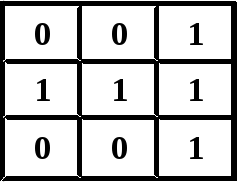
\includegraphics[scale=.7]{./Figures/EX3}\label{fig:EX:3}} 
\\
\subfigure[Cruz de $5x5$.]{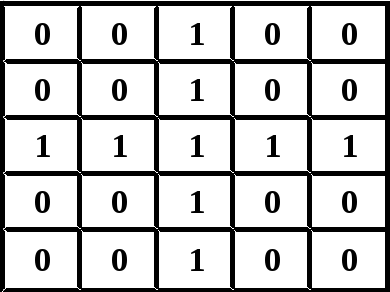
\includegraphics[scale=.7]{./Figures/EX2}\label{fig:EX:2}}
\caption{Ejemplos de elementos estructurales} \label{fig:EX}
\end{figure} 

Existen distintas operaciones morfológicas, las principales o básicas son la dilatación y erosión las cuales se explican enseguida junto con la apertura y el cierra. 
 
\subsection{Dilatación}\label{Dilatation}

La dilatación es una operación que añade pixeles a la orilla de los objetos que se encuentran en la imagen. La dilatación se define como:  
$$S \oplus EX = \lbrace S|EX_S \subseteq S \rbrace$$  
donde $EX_S$ es el elemento estructural trasladado con la imagen. 

\subsection{Erosión}\label{OMerosion}

La erosión remueve pixeles a la orilla de los objetos que se encuentran en la imagen. La erosión se define como: 
$$S \ominus EX = \lbrace S|EX_S \subseteq S \rbrace$$ 
donde $EX_S$ es el elemento estructural trasladado con la imagen. 

\subsection{Apertura}\label{Opening} 

La operación apertura abre huecos entre objetos conectados por un enlace delgado de pixeles.  

$$S \circ EX = (S \ominus EX) \oplus EX $$

\subsection{Cierre}\label{Cierre}

La operación cierre elimina huecos pequeños  y rellena huecos en las
$$S \bullet EX = (S \oplus EX) \ominus EX $$

\section{Casco convexo y defectos de convexidad}\label{sec:Convexhull} 

Antes de definir el casco convexo se presenta la definición de conjunto convexo. 
 

Sea $C$ un conjunto de puntos en el plano Euclidiano, el casco convexo es el conjunto convexo más pequeño que contiene a todos los puntos en $C$. 

Los defectos de convexidad de un con casco convexo, es el conjunto de puntos que no pertenecen al casco convexo. El defecto es el espacio entre la linea y el objeto  



\section{M\'aquinas de soporte vectorial}\label{sec:SVM} 

$N$ puntos de entrenamiento de dimensión $D$, dos clases distintas $y_i=-1$
o $+1$ es decir: 

${x_i,y_i}$ donde $i=1, \cdots ,N$, $y\in{-1,1}$, $x \in \Re^D$  

Hiperplano óptimo 
 
$$ w \cdot x + b = 0$$ 

donde $w$ es la normal al hiperplano, $\frac{b}{|w|}$ es la distancia perpendicular desde el hiperplano al origen.   

$$ w \cdot x + b = +1 \textrm{ para } y_i=+1$$ 
$$ w \cdot x + b = -1 \textrm{ para } y_i=-1$$ 

Maximizar el margen, encontrar el mínimo de $w$.  

$Min$ $\Vert w \Vert$ tal que $y_i(w \cdots x_i + b) -1 \geq 0$
 
\begin{figure}[!h]
\begin{center}
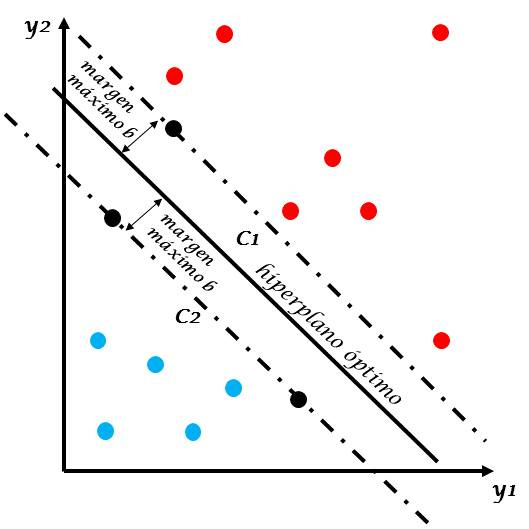
\includegraphics[scale=.3]{./Figures/maquinaSoporte.jpg}
\end{center}
\caption{Clasificación de maquina de soporte usando kernel lineal}
\label{fig:SVM}
\end{figure} 


\newpage
%%=====================================================
